

\subsection{Lattice setup}
    Gauge configurations in this work were obtained from the ensemble A40.24 which has been generated using $N_f = 2 + 1 + 1$ quark flavors. Details can be looked up in \cite{guage_configurations}.
    
    \begin{table}[h]
        \centering
        \begin{tabular}{lllllll}
        \hline
        \multicolumn{1}{|c|}{$\#$ used configurations} & \multicolumn{1}{c|}{$\beta$} & \multicolumn{1}{c|}{$\kappa$} & \multicolumn{1}{c|}{$a\mu_I$} & \multicolumn{1}{c|}{$a\mu_\sigma$} & \multicolumn{1}{c|}{$a\mu_\delta$} & \multicolumn{1}{c|}{$(L/a)^3 \times T$} \\ \hline
        \multicolumn{1}{|c|}{11} & \multicolumn{1}{c|}{3.9} & \multicolumn{1}{c|}{0.160856} & \multicolumn{1}{c|}{0.0040} & \multicolumn{1}{c|}{??} & \multicolumn{1}{c|}{??} & \multicolumn{1}{c|}{$24^3 \times 48$} \\ \hline
                               &                       &                       &                       &                       &                       &                       \\
                               &                       &                       &                       &                       &                       &                      
        \end{tabular}
        \caption{Parameters of gauge configurations used}
        \label{table_gauge_params}
    \end{table}
    % TODO explanation
    
\subsection{Meson masses}
    To investigate the accuracy and usefulness of the method of distillation described in this thesis comutations of charmonium state correlation functions where performed. These enable one to test different configurations of eigenvectors in relatively short times compared to the use of light doublet states. Beside the number of gauge configurations the number of eigenvectors can be arbitrarily set. In this section I will present the results for 1, 2, 5 and 10 eigenvectors on the 11 gauge configurations mentioned in the previous section.\\
    
    \begin{figure}[H]
        \centering
        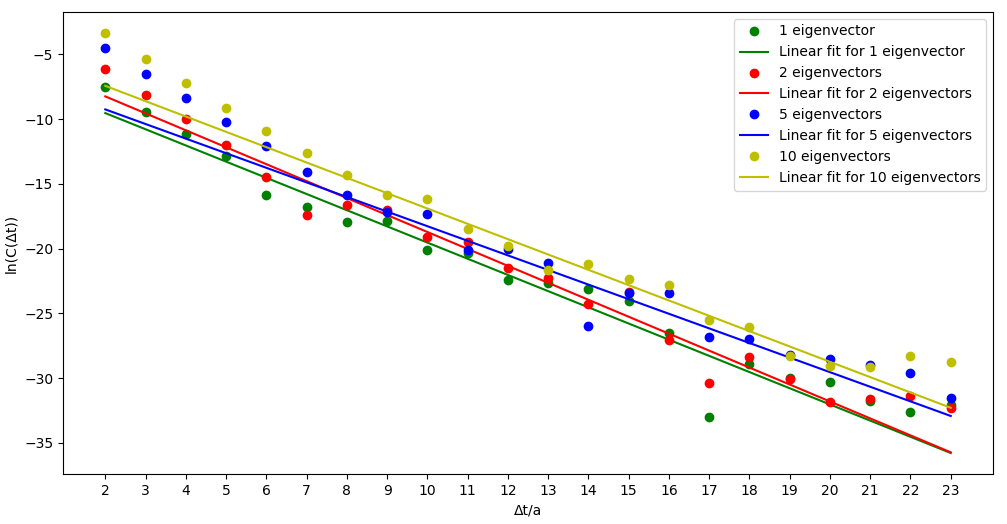
\includegraphics[width=1\textwidth]{images/1_2_5_10_evs_log.png}
        \caption{Combined results for 1, 2, 5 and 10 eigenvectors}
        \label{1_2_5_10_evs_log}
    \end{figure}
    
    \noindent
    In all computations the following creation operator was used:
    \begin{equation}
        \Operator(t) = \bar{\chi}^{(c)}(t)\gamma_5\chi^{(c)}(t)
    \end{equation}
    Therefore the resulting meson has quantum numbers $0(0^-)$ \cite{masses_of_D_mesons}. This was achieved by using for both propagators $(D^{-1(f)})$ the same flavor $f$. This approach reduced the amount of inversions that had to be calculated significantly. For the same reason a charmonium state was chosen in contrast to e.g. the calculation of a pion mass. Inversions for particles with higher masses converge significantly faster.
    
    To compute the mass of the charmonium state the mean value of all configurations for one value of $\Delta t$ were computed and a simple linear function was fitted to $ln(C(\Delta t))$. The results for 1, 2, 5 and 10 eigenvectors can be seen in figure \ref{1_2_5_10_evs_log}. One can see the similar shapes of all four results. Because the exponential nature of the correlation function only holds for $\Delta t \rightarrow \infty$ only a few points were chosen to be fitted. In figure \ref{1_2_5_10_evs_log_separate} one can see the four results side by side. The points which were used to fit the linear function are colored differently.
    
    The masses of these four simulations are shown in table \ref{meson_masses}, the errors were calculated using the \textit{Jackknife} \cite{jackknife} method.
    \begin{table}[h]
            \centering
            \begin{tabular}{|c|c|}
            \hline
            \multicolumn{1}{|c|}{Number of eigenvectors} & \multicolumn{1}{c|}{Mass (MeV)} \\ \hline
             1 & $3082 \pm 255$\\
             2 & $3227 \pm 215$\\
             5 & $2780 \pm 91$\\
             10& $2919 \pm 88$\\
              \hline
            \end{tabular}
            \caption{Calculated masses for the charmonium state}
            \label{meson_masses}
        \end{table}
    
    
    
    \begin{figure}[H]
        \centering
        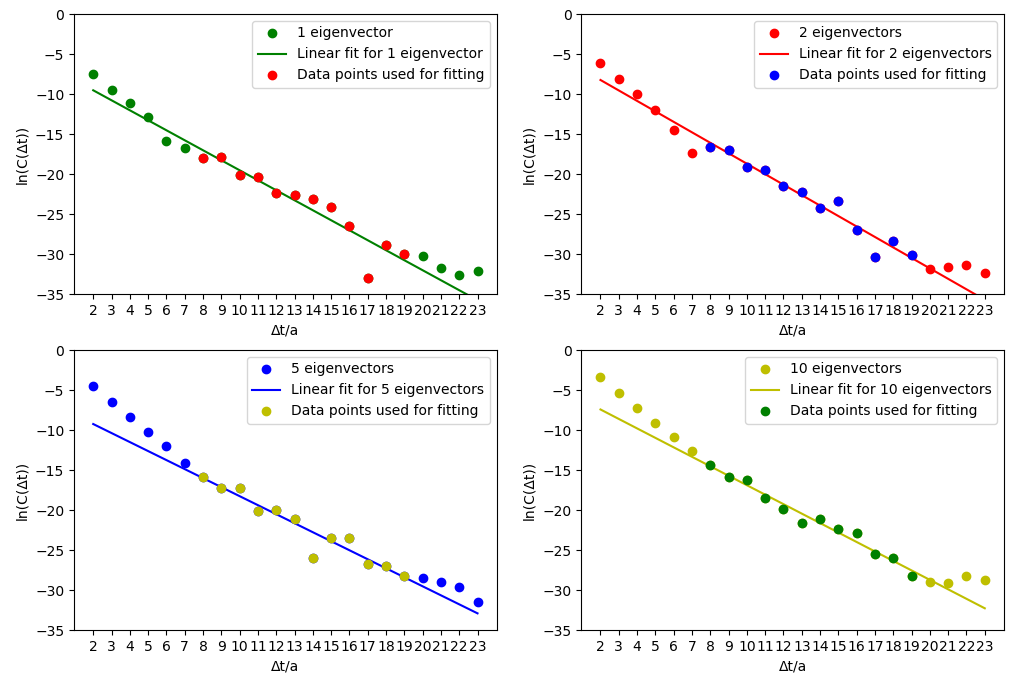
\includegraphics[width=1\textwidth]{images/1_2_5_10_evs_side.png}
        \caption{Logarithmic results for 1, 2, 5 and 10 eigenvectors. The data points used for fitting are colored differently.}
        \label{1_2_5_10_evs_log_separate}
    \end{figure}